
\Chainmail assertions (details in appendix \ref{sect:standard}) consist of (pure) expressions \e, comparisons between expressions, classical
assertions about the contents of heap and stack, the usual logical
connectives, as well as our holistic concepts.
In this section we focus on the novel,
 holistic, features of \Chainmail (permission, control, time, space, and viewpoint),
as well as our wish to support some form of recursion while keeping the logic of assertions classical.
% SD I removed the belowas it is no longer true here. % don't understand what you mean so i have deleted the next paragraph
%\sdN{Expressions include variables, field lookup, and the execution of (pure) ghost methods. 
%This  supports recursion at the level of expressions; therefore, the value of  an expression  may be
% undefined (either because of infinite recursion, or because the expression accessed undefined fields or variables). 
 %Assertions of the form   $\e$=$\e'$ are satisfied only if both $\e$ and $\e'$ are defined. Because we do not support 
% recursion at the level of assertions, assertions form a classical logic (\eg $\A \vee \neg\A$ is a tautology)
%}
%Assertions support the comparison of expressions, and the usual logical connectives
%(Appendix, section \ref{sect:standard}), as well as the usual connectives discussed below.
%We now define the syntax and semantics of expressions and holistic assertions.
%\sd{The novel, holistic, features of \Chainmail (permission, control, time, space, and viewpoint),
%as well as our wish to support some form of recursion while keeping the logic of assertions classical,  introduced 
%challenges, which we discuss in this section.}

\subsection{Syntax and Semantics}
 
We now define the syntax and semantics of expressions and holistic assertions.
\sd{The novel, holistic, features of \Chainmail (permission, control, time, space, and viewpoint),
as well as our wish to support some form of recursion while keeping the logic of assertions classical,  introduced 
challenges, which we discuss in this section.}

 \subsection{Syntax of Assertions}

\begin{definition}[Assertions]  Assertions consist of (pure) expressions \e, classical assertions about the contents of heap/stack, the usual logical  connectives, as well as our holistic concepts.
\label{def:assertions}
 \[
 \begin{array}{lcl}
  ~  \\
 \prg{v}  &\BBC&    \kwN{true}   ~\SOR~  \kwN{false}   ~\SOR~  \kwN{null}  ~\SOR~  \alpha ~\SOR~ \prg{x} \\
  ~  \\
 \SE  &\BBC&    \prg{v}\ ~\SOR~ \SE=\SE    ~\SOR~ \kwN{if}\, \SE\,   \kwN{then}\,  \SE\,    \kwN{else}\, \SE    ~\SOR~  \SE.\f\lp\ \SE^* \ \rp\\
     \\
 \A &\ \BBC   &   \SE \   \mid \  \SE=\SE  \mid \   \SE:\prg{ClassId}  \ \mid \
    \SE\in\prg{S}   \mid  \  \\
    &
  &  \A \rightarrow \A  \ \mid\  \     \A \wedge \A  \ \mid\  \  \A \vee \A  \ \mid\  \ \neg A   \ \mid \ \\
  & &  \forall \alpha.\A  \ \mid \  \forall \prg{S}:SET.\A  \ \mid  \  \exists \alpha.\A  \ \mid \  \exists \prg{S}:SET.\A  \  \ \mid \\
 &    &  \CanAccess {\alpha_1} {\alpha_2} \ \mid\  \ \Changes e 
           \ \mid\  \Calls {\alpha_1}  {\prg{m}} {\alpha_2}  {\prg{v}^*}\mid\\          
&    &  \Next \A  \ \mid \   \Future \A \ \mid \  \Prev \A   \ \mid \ \Past \A \ \mid \\  
 &    &        \Using \SF  \A  \ \mid \  \External \alpha\\
 \\
 \x, \f, \m &\BBC&  \prg{Identifier}  ~ \\
\end{array}
\]
\end{definition}
 
Expressions support calls with parameters  ($\e.\f(\e^*)$); these are calls to ghostfield
functions. This  supports recursion at the level of expressions; therefore, the value of  an expression  may be
undefined (either because of infinite recursion, or because the expression accessed undefined fields or variables). 
Assertions of the form   $\e$=$\e'$ are satisfied only if both $\e$ and $\e'$ are defined. Because we do not support 
recursion at the level of assertions, assertions form a classical logic (\eg $\A \vee \neg\A$ is a tautology).
 
We will discuss evaluation of expressions in section \ref{sect:expressions}, standard assertions about heap/stack and logical
 connectives in \ref{sect:standard}. 
 We will discuss the treatment of  permission, control, space, and viewpoint  in 
the main text in  Defs.~\ref{def:valid:assertion:access}-\ref{def:valid:assertion:space}  in section \ref{sect:pcsv} %HARD
the treatment of time in Defs. \ref{def:reduction:constrained}, \ref{def:valid:assertion:time} in the main text, section \ref{sect:time},
We will discuss properties of assertions in Lemmas \ref{lemma:classic}-\ref{lemma:classic:two}.
 The judgement $\M\mkpair \M', \sigma_0 ,  \sigma  \models \A$ expresses that $\A$ holds in  $\M\mkpair \M'$ and $\sigma$, and 
while $\M\mkpair \M', \sigma_0 , \sigma  \not\models \A$  expresses that $\A$ does not hold  in  $\M\mkpair \M'$ and $\sigma_0,\sigma$.
 
\subsection{Values of Expressions}
\label{sect:expressions}

The value  of  an expression  is described through judgment $ \M,\, \sigma, \SE \ \hookrightarrow\  v$,
defined in Fig.~\ref{fig:ValueSimpleExpressions}.
We use the configuration, $\sigma$, to read the contents of the top stack frame
% value of variables defined in the stack frame
(rule ${\sf {Var\_Val}}$) or the contents of the heap (rule
${\sf {Field\_Heap\_Val}}$). We use the module, \M, to find the  ghost field declaration corresponding to the
ghost field being used. 

The treatment of fields and ghost fields is described in rules ${\sf {Field\_Heap\_Val}}$,\\  ${\sf {Field\_Ghost\_Val}}$ and 
${\sf {Field\_Ghost\_Val2}}$.  If the field \f~ exists in the heap, then its value is returned (${\sf {Field\_Heap\_Val}}$). 
Ghost field reads, on the other hand, have the form $\e_0.\f(\e_1,...\e_n)$, and their value is
described in rule ${\sf {Field\_Ghost\_Val}}$:
%
The lookup function $\mathcal G$  (defined in the obvious way in the Appendix, Def.~\ref{def:lookup})
returns the expression constituting the body for that ghost field, as defined in the class of $\e_0$.
We return  that expression
evaluated in a configuration where the formal parameters have been substituted by the values of the actual
parameters.

Ghost fields support recursive definitions. For example, imagine a module $\M_A$ with
a class \prg{Node} which has a field called \prg{next}, and which 
had a ghost field \prg{last}, which finds  the last \prg{Node} in a sequence
and is defined recursively as \\
$~ \strut \hspace{.1cm}$ \ \ \ \prg{if}\ \ \prg{this.next}=\prg{null}\  \prg{then} \ \prg{this} \ \prg{else} \ \prg{this.next.last},\\
and another ghost field \prg{acyclic}, which expresses that a sequence is acyclic,
defined recursively as \\
$~ \strut \hspace{.1cm}$ \ \ \ \prg{if}\ \ \prg{this.next}=\prg{null}\  \prg{then} \ \prg{true} \ \prg{else} \ \prg{this.next.acyclic}.

The relation $ \hookrightarrow$ is partial. 
For example, assume   a configuration
$\sigma_A$ where
\prg{acyc} points to a \prg{Node} whose field \prg{next} has value \prg{null}, and   
\prg{cyc} points to a \prg{Node} whose field \prg{next} has the same value as \prg{cyc}. Then,   
$\M_A,\sigma_A,\,\prg{acyc.acyclic}  \ \hookrightarrow\  \prg{true}$, but we would have no value for 
$\M_A,\sigma_A,\, \prg{cyc.last}  \ \hookrightarrow\  ...$, nor for
$\M_A,\sigma_A,\, \prg{cyc.acyclic}  \ \hookrightarrow\  ...$.

Notice also that for an expression of the form  
\prg{\e.\f}, both ${\sf {Field\_Heap\_Val}}$ and ${\sf {Field\_Ghost\_Val2}}$ could be applicable: rule ${\sf {Field\_Heap\_Val}}$
will be applied if \prg{f} is a field of the object at \prg{e}, while rule ${\sf {Field\_Ghost\_Val}}$
will be applied if \prg{f} is a ghost field of the object at \prg{e}. We expect the set of fields and ghost fields in a 
given class to be disjoint.
This allows a specification to be agnostic over whether a field is a physical field or just ghost information.
For example, assertions (1) and (2) from  section  \ref{sect:motivate:Bank}
 talk about the \prg{balance} of an \prg{Account}. 
In module $\M_{BA1}$ (Appendix~\ref{Bank:appendix}), where we keep the balances in the account objects, this is a physical field. 
In $\M_{BA2}$ (also in Appendix~\ref{Bank:appendix}), where we keep the
balances in a ledger, this is ghost information.  

\begin{figure*}
{
$\begin{array}{l}
\begin{array}{llll}
\inferenceruleN {True\_Val} {
}
{
 \M,\, \sigma, \kwN{true} \ \hookrightarrow\  \kwN{true}
}
& 
\inferenceruleN {False\_Val} {
}
{
 \M,\, \sigma, \kwN{false} \ \hookrightarrow\  \kwN{false}
}
&
\inferenceruleN  {Null\_Val} {
}
{
 \M,\, \sigma, \kwN{null} \ \hookrightarrow\  \kwN{null}
}
&
\inferenceruleN {Addr\_Val %{Had to switch old \textit{Var_Val} rule for \textit{Addr_Val}}
} {
\alpha : \text{Address}
}
{
 \M,\,  \sigma, \alpha \ \hookrightarrow\   \alpha
}
\end{array}
\\ \\
\begin{array}{lll}
\begin{array}{l}
\begin{array}{ll}
\inferenceruleExact{\SP\SP\SP}{Var\_val} {
 \interp {\x}{\sigma} = v
}
{
 \M,\, \sigma, \x  \ \hookrightarrow\   v
}

&
\inferenceruleExact{\SP}{Field\_Ghost\_Val2} {
 \M,\, \sigma, \SE.\f \lp \rp \ \hookrightarrow\   v
}
{
 \M,\, \sigma, \SE.\f   \ \hookrightarrow\   v
}
\end{array}
\\
\\
\inferenceruleNM{Field\_Heap\_Val} {
 \M,\,  \sigma, \SE \ \hookrightarrow\   \alpha \hspace{1.5cm} 
 \sigma(\alpha,\f)=v
}
{
 \M,\, \sigma, \SE.\f  \ \hookrightarrow\   v
}
\end{array}
& &
\inferenceruleNM{Field\_Ghost\_Val}
{
%~ \\
 \M,\, \sigma, \SE_0   \ \hookrightarrow\  \alpha \hspace{1.9cm} \sigma = (\_, \chi) 
\\
 \M,\, \sigma, \SE_i  \ \hookrightarrow\   v_i\ \ \ \ i\in\{1..n\}
 \\
{\mathcal{G}}
(\M, {\ClassOf {\alpha} {\sigma}}, {\f}) \  =  
\ \f\lp \p_1, \ldots \p_n \rp \lb\ \SE \ \rb
  \\

\phi = (\_, (\this\mapsto\alpha, \p_1\mapsto v_1, .... \p_n\mapsto v_n))\\  
  
  \M,\,(\phi, \chi), \SE'    \hookrightarrow\   v  \hspace{1.2cm} \SE' = f_{\mathcal G}(\SE)
 }
{
 \M,\,  \sigma, \ \SE_0.\f \lp \SE_1,....\SE_n\rp \hookrightarrow   \ v
}
\\ \\
\inferenceruleNM{If\_True\_Val} 
{
 \M,\,  \sigma, \SE \ \hookrightarrow\   \prg{true}  \\
   \M,\,  \sigma, \SE_1 \ \hookrightarrow\   v  
}
{
 \M,\, \sigma, \kwN{if}\ \SE\  \kwN{then} \ \SE_1 \ \kwN{else} \ \SE_2\  \hookrightarrow  \ v
}
& &
\inferenceruleNM {If\_False\_Val} 
{
 \M,\,  \sigma, \SE \ \hookrightarrow\   \prg{false}  \\
   \M,\,  \sigma, \SE_2 \ \hookrightarrow\   v  }
{
 \M,\, \sigma, \kwN{if}\ \SE\  \kwN{then} \ \SE_1 \ \kwN{else} \ \SE_2\  \hookrightarrow\  v
}
\\ \\ 
\inferenceruleNM {Equals\_True\_Val} 
{
 \M,\,  \sigma, \SE_1 \ \hookrightarrow\    v \\
   \M,\,  \sigma, \SE_2 \ \hookrightarrow\     v 
}
{
 \M,\, \sigma, \SE_1 =  \SE_2 \hookrightarrow \prg{true}
}
& &
\inferenceruleNM {Equals\_False\_Val} 
{
 \M,\,  \sigma, \SE_1 \ \hookrightarrow\    v \\
   \M,\,  \sigma, \SE_2 \ \hookrightarrow\     v' \hspace{2cm}  v\neq v'
}
{
 \M,\, \sigma, \SE_1 =  \SE_2 \hookrightarrow \ \prg{false}
}
\end{array}
\end{array}
$}
\caption{Value of  Expressions}
\label{fig:ValueSimpleExpressions}
\end{figure*}

\subsection{Satisfaction of Assertions - Standard}
\label{sect:standard}
\sd{
We now define the semantics of assertions involving expressions, the heap/stack, and logical connectives.
The semantics are unsurprising, except, perhaps the relation between validity of assertions and the values of
expressions.
}


 \begin{definition}[Interpretations for simple expressions]

For a runtime configuration, $\sigma$,    variables $\x$ or \SF, we define its interpretation as follows:

\begin{itemize}
  \item
  $\interp {\x}{\sigma}$ $ \triangleq$ $\phi(\x)$  \ \ if \ \ $\sigma$=$(\phi\cdot\_,\_)$
  \item
    $\interp {\x.\f}{\sigma}$ $ \triangleq$ $\chi(\interp {\x}{\sigma},\f)$  \ \ if \ \ $\sigma$=$(\_,\chi)$
   \end{itemize}
\end{definition}   


\begin{definition}[ Basic Assertions] For modules $\M$, $\M'$,  configuration $\sigma$,  we define$:$
%validity of basic assertions: 
\label{def:valid:assertion:basic}
\begin{itemize}
\item
$\M\mkpair \M', \sigma_0 ,\sigma \models\SE$ \IFF   $ \M,\,  \sigma, \SE \ \hookrightarrow\   \prg{true}$ 
\item
$\M\mkpair \M',\sigma_0 , \sigma \models\SE=\SEPrime$ \IFF there exists a value $v$ such that  $\M,\,  \sigma, \SE \ \hookrightarrow\   v$  and $ \M,\,  \sigma, \SEPrime \ \hookrightarrow\   v$.
           \item
$\M\mkpair \M',\sigma_0 , \sigma \models\SE:\prg{ClassId}$ \IFF there exists an address $\alpha$ such that \\
$\strut ~ $ \hspace{2in} \hfill   
 $ \M,\,  \sigma, \SE \ \hookrightarrow\   \alpha$, and $\ClassOf{\alpha}{\sigma}$ = \prg{ClassId}.
\item
$\M\mkpair \M',\sigma_0 , \sigma \models \SE\in \prg{S}$ \IFF there exists a value $v$ such that 
 $ \M,\,  \sigma, \SE \ \hookrightarrow\   v$, and $v \in \interp{\prg{S}}{\sigma}$.
\end{itemize}
\end{definition}

Satisfaction of assertions which contain expressions is predicated on termination of these expressions.
Continuing our earlier example, given any initial configuration $\sigma_0$,  
$\M_A\mkpair \M', \sigma_0,\sigma_A \models \prg{acyc.acyclic}$ holds for any $\M'$, while $\M_A\mkpair \M', \sigma_0,\sigma_A \models \prg{cyc.acyclic}$
does not hold, and $\M_A\mkpair \M', \sigma_0,\sigma_A \models \prg{cyc.acyclic}=\prg{false}$ does not hold either.
In general, when $\M\mkpair \M', \sigma  \models \prg{e}$ holds,  then $\M\mkpair \M', \sigma  \models \prg{e}=\prg{true}$ holds too.
But when $\M\mkpair \M', \sigma  \models \prg{e}$ does not hold, this does \emph{not} imply that $\M\mkpair \M', \sigma  \models \prg{e}=\prg{false}$ holds.
Finally, an assertion of the form $\e_0=\e_0$ does not always hold; for example,   $\M_A\mkpair \M', \sigma_A \models \prg{cyc.last}=\prg{cyc.last}$ does not hold.

% \subsubsection{Logical connectives, quantifiers, space and control} 
We now define satisfaction of assertions which involve logical connectives and existential or universal quantifiers, in the standard way:


\begin{definition}[Assertions with logical connectives and quantifiers]  
%We now consider 
\label{def:valid:assertion:logical}
For modules $\M$, $\M'$, assertions $\A$, $\A'$, variables \prg{x}, \prg{y}, \prg{S},  and configurations $\sigma_0$ $\sigma$, we define$:$
\begin{itemize}
\item
$\M\mkpair \M',\sigma_0 ,  \sigma \models \forall \prg{S}:\prg{SET}.\A$ \IFF  $\M\mkpair \M', \sigma_0 ,  \sigma \models  \A[\prg{S}/\prg{R}]$ \\
$\strut ~ $ \hfill for all sets of addresses $R\subseteq dom(\sigma)$.
\item
$\M\mkpair \M',\sigma_0 ,\sigma \models \exists \prg{S}:\prg{SET}\!.\,\A$ \IFF  $\M\mkpair \M', \sigma_0  ,  \sigma \models  \A[\prg{S}/\prg{R}]$ \\
 $\strut ~ $ \hfill  for some set of addresses $R\subseteq dom(\sigma)$.
\item
$\M\mkpair \M',\sigma_0 ,\sigma \models \forall \alpha.\A$ \IFF
$\M\mkpair \M',\sigma_0 ,\sigma \models  \A[\alpha/\alpha']$ \ for all  $\alpha'\in dom(\sigma)$.
\item
$\M\mkpair \M',\sigma_0 , \sigma \models \exists \alpha.\A$ \IFF
$\M\mkpair \M', \sigma_0 , \sigma \models  \A[\alpha/\alpha']$\ for some  $\alpha
\in dom(\sigma)$.
\item
$\M\mkpair \M',\sigma_0 , \sigma \models \A \rightarrow \A' $ \IFF  $\M\mkpair \M',\sigma_0 ,   \sigma \models \A $ implies $\M\mkpair \M',\sigma_0 ,   \sigma \models \A' $
\item
$\M\mkpair \M',\sigma_0 ,  \sigma \models  \A \wedge \A'$   \IFF  $\M\mkpair \M',\sigma_0 ,   \sigma \models  \A $
and $\M\mkpair \M',\sigma_0 ,   \sigma \models  \A'$.
\item
$\M\mkpair \M',\sigma_0 ,  \sigma \models  \A \vee \A'$   \IFF  $\M\mkpair \M', \sigma_0 , \sigma \models  \A $
or $\M\mkpair \M',\sigma_0 ,  \sigma \models  \A'$.
\item
$\M\mkpair \M',\sigma_0 ,  \sigma \models  \neg\A$   \IFF  $\M\mkpair \M',\sigma_0 ,  \sigma \models  \A $
does not hold.
\end{itemize}
\end{definition}


Satisfaction is not preserved with growing configurations; for example, the assertion $\forall \x. [\ \x : \prg{Account} \rightarrow \x.\prg{balance}>100\ ]$ 
may hold in a smaller configuration, but not hold in an extended configuration. 
Nor is it preserved with configurations getting smaller; consider \eg $\exists \x. [\ \x : \prg{Account} \wedge \x.\prg{balance}>100\ ]$.

\noindent
Again, with our earlier example,  
$\M_A\mkpair \M', \sigma_0 , \sigma_A \models \neg (\prg{cyc.acyclic}=\prg{true})$    and  
$\M_A\mkpair \M', \sigma_0 , \sigma_A \models  \neg (\prg{cyc.acyclic}=\prg{false})$, 
and also 
$\M_A\mkpair \M', \sigma_0 , \sigma_A \models  \neg (\prg{cyc.last}=\prg{cyc.last})$
hold.

\Chainmail quantifies over addresses instead of local variables. Since \Chainmail assertions are invariants over modules, local variable names have no consistent denotation as the stack frame changes during execution. Previous work on \Chainmail exclusively used variables in assertions, including for quantification \cite{FASE}. Aside from being less clear, as assertions generally refer to objects meeting some property, rather than the value at a certain name, using local variables also complicated the handling of temporal assertions, as discussed in section~\ref{sect:time}.

\subsection{Satisfaction of Assertions - Access, Control, Space, Viewpoint}
\label{sect:pcsv} 
%We now consider the assertions which involve access:

\textit{Permission} expresses that an object has the potential to call
methods on another object, and to do so directly, without  help from any
intermediary object. This is the case when both are the same instance---the addresses therefore being identical; or the first object has a field pointing to the second object; or
the first object is the receiver of the currently executing method and the second object is one of the 
arguments or a local variable. Interpretations of variables and paths, $\interp {...} {\sigma}$, are defined
in the usual way (appendix Def.~\ref{def:interp}).


\begin{definition}[%Satisfaction of  Assertions about 
Permission]  \label{def:valid:assertion:access}
\Mrr{For any modules $\M$, $\M'$,  addresses $\alpha$ and $\alpha'$, we define:}
\begin{itemize}
\item
$\M\mkpair \M', \sigma_0 , \sigma \models  \CanAccess{\alpha_1}{\alpha_2}$  \IFF  
%\begin{itemize}
%\item
%$\alpha_1$=$\alpha_{2}$, \ \ or
%\item
%$\interp {\x.\f} {\sigma}$=$\interp {\y} {\sigma}$, \  \ for some field \prg{f},  \ \ or
%\item
%$\interp {\x} {\sigma}$=$\interp {\this} {\sigma}$ and
%  $\interp {\y} {\sigma}$=$\interp {\z} {\sigma}$,\ \ \ 
%for some variable \z\ and  \z\ appears in  $\sigma$.\prg{contn}.
% \end{itemize}
%$\M\mkpair \M', \sigma_0 , \sigma \models  \CanAccess{\alpha_1}{\alpha_2}$   \IFF   
\begin{itemize}
\item
$\alpha_1$=$\alpha_{2}$, \ \ or
\item
$\sigma(\alpha_1,\f) $=${\alpha_2}$, \  \ for some field \prg{f},  \ \ or
\item
${\alpha_1}$=$\interp {\this} {\sigma}$ and
  ${\alpha_2}$=$\interp {\x} {\sigma}$, \ \ for some variable \x
  %,\ \ \ 
%for some variable \x\ and  \x\ appears in  $\sigma$.\prg{contn}.
\end{itemize}
\end{itemize}
\end{definition}



\noindent 
%Therefore, $\CanAccess{\prg{x}}{\prg{y}}$ expresses that \x\, has a {\em direct} path to \y.
%It says that in the current frame,
%either \x~and \y\ are  aliases, or \x~points to an object which has a field
% whose value is the same as that of \y, or \x\, is the currently executing object and \y\, is
In the last disjunct the interpretation of \x\ in the configuration ensures it is a parameter or local variable.

\vspace{.2cm} \noindent
\textit{Control} expresses which object is the process of making a function call on another object and
with what arguments. The relevant information
\sophia{is} stored in the continuation (\prg{cont}) on the top frame.

\begin{definition}[%Satisfaction of  Assertions about 
Control]  \label{def:valid:assertion:control}
For any modules $\M$, $\M'$,  \Mrr{addresses $\alpha$, $\alpha'$, $\alpha_1,...\alpha_n$}, we define$:$
\begin{itemize}
   \item
$\M\mkpair \M', \sigma_0 , \sigma \models  \Calls {\alpha}  {\prg{m}} {\alpha'}  {\alpha_1,...\alpha_n}$ \IFF \ \ \ 
\begin{itemize}
\item
$\interp{\prg{this}}{\sigma}$=$\alpha$, \ and
\item
% $\strut ~ \hspace{2.1in} $  
$\sigma.\prg{contn}$=${\x.\m(\y_1,..\y_n);\_}$,\ \ \ for some  $\x$,$\y_1$,... $\y_n$, \ and
\item
%  $\strut ~ \hspace{2.1in} $ 
 $\interp{\prg{x}}{\sigma}$=$\alpha'$,\ \ \ and \ \ \ 
  $\interp{{\prg{y}_i}}{\sigma}=\alpha_i$, for all  $i$.
 \end{itemize}
  \end{itemize}
\end{definition}

\noindent 
Thus, $\Calls {\alpha}  {\prg{m}} {\alpha'}  {{\alpha_1,...\alpha_n}}$ expresses that there is about to be a call from $\alpha_1$ to the method \m\ on object $\alpha'$ , given objects $\alpha_1,...\alpha_n$. If these are named \y, and $\z_1,...\z_n$ respectively, then $\y.\m(\z_1,...\z_n)$ will be executed next, and the current caller \this\ is $\alpha$.
 

\vspace{.2cm} \noindent
\textit{Viewpoint} concerns whether an object is viewed as belonging to the internal module, determined by the class of the object.

 \begin{definition}[%Satisfaction of  Assertions about 
Viewpoint]  \label{def:valid:assertion:view}
For any modules $\M$, $\M'$, and addresses $\alpha$, $\alpha'$, we define
\begin{itemize}
 \item
$\M\mkpair \M', \sigma_0 , \sigma \models \External {\alpha}$ 
  \IFF
 $\ClassOf {\alpha} {\sigma} \notin dom(\M)$
\item
$\M\mkpair \M',\sigma_0 ,  \sigma \models \Internal {\alpha}$ 
  \IFF
  $\ClassOf {\alpha} {\sigma} \in dom(\M)$
%\item
%$\M\mkpair \M',\sigma_0 ,  \sigma \models \prg{private} \langle {\alpha, \alpha'} \rangle$ 
%  \IFF
%  $\M\mkpair \M',\sigma_0 , \sigma \models \alpha.\texttt{private}\prg{(}\alpha'{)}$
\end{itemize}
\end{definition}
\noindent 


 
\vspace{.2cm} 

\noindent
\textit{Space} asserts that some property \A\ holds in a configuration whose objects are restricted to those
from a given set \SF. This way we can express that the objects from the set \SF\ have authority over the assertion \A.

In order to define validity of $\Using {\A} {\prg{S}}$ in a configuration $\sigma$, 
we first define a restriction operation,  $\restrct {\sigma}{\prg{S}}$ which restricts the objects from $\sigma$ to only those
from $\SF$.

\begin{definition}[Restriction of Runtime Configurations]  \label{def:restrict}
The restriction operator~$\;\restrct{} {} $ applied to a runtime configuration $\sigma$ and a variable  \prg{S} is defined as follows:
 \label{def:config:restrct}
 $~ $
\begin{itemize}
\item
$\restrct {\sigma}{\prg{S}}  \triangleq  (\sd{\psi}, \chi')$, \ if \  $\sigma$=$(\psi,\chi)$, \    $dom(\chi')=\prg{S}$, and   
% \\ $\ \strut \ \ \hspace{1.2in} $
 $\forall \alpha\!\in\!dom(\chi').\chi(\alpha)=\chi'(\alpha)$.
\end{itemize}
\end{definition}

\begin{tabular}{cc}
 \begin{minipage}{0.45\textwidth}
\sd{For example, if we take $\sigma_2$ from Fig.~\ref{fig:BankAccountDiagrams} in Section \ref{sect:motivate:Bank},
and restrict it with some set $\SF_4$ such that $\SF_4=\{ 91, 1, 2, 3, 4, 11 \}$,
then the restriction $\restrct {\sigma_2}{\prg{S}_4}$ will look as on the right.}
  \end{minipage}
 &  
 \begin{minipage}{0.45\textwidth}
% $\restrct {\sigma_2}{\prg{S}_4}$\\
  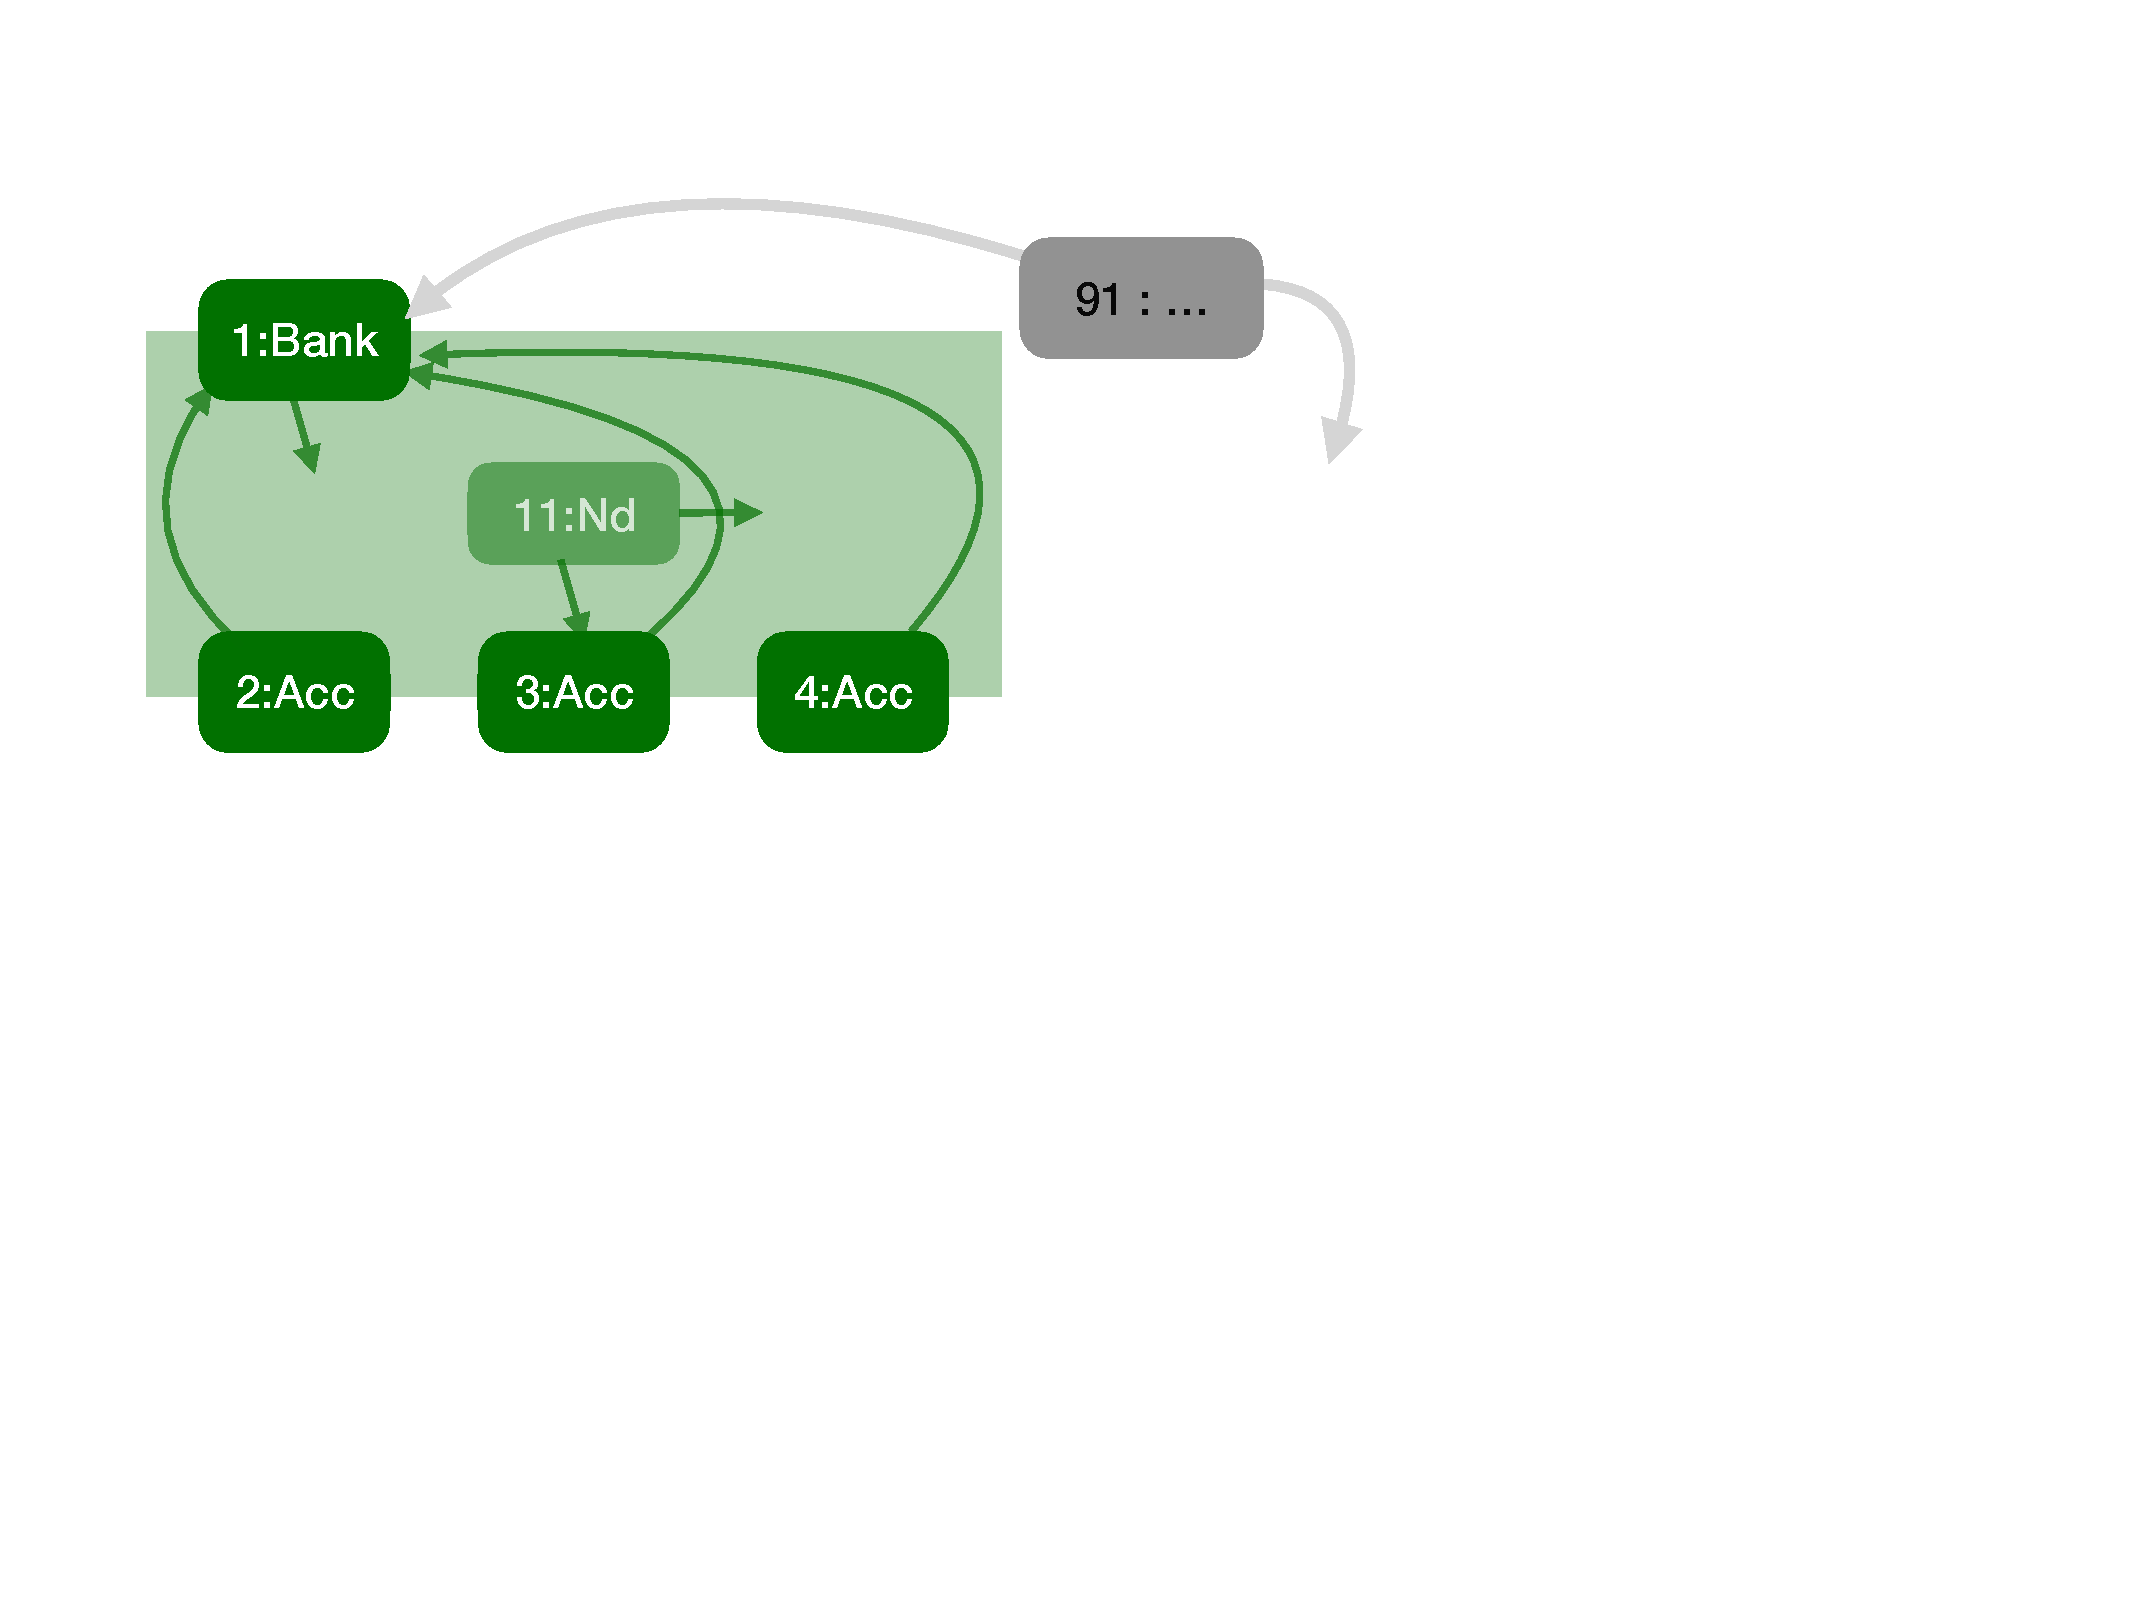
\includegraphics[width=\linewidth, trim=55  330 320 60,clip]{diagrams/BankAccount_version_2a.pdf}
  \Description{A green zone with 5 nodes in it: one bank object, 3 account objects, and one list node, labelled 11. A further node is outside the green zone, labelled 91.}
   \end{minipage}
\end{tabular}
 
\sd{Note in the diagram above the dangling pointers at objects $1$,  $11$, and $91$ - reminiscent of the separation
of heaps into disjoint subheaps, as provided by the 
$*$ operator in separation logic \cite{Reynolds02}. The difference is that in separation logic, the 
separation is provided through the assertions, where $\A * \A'$ holds in any heap  which can be split into
disjoint $\chi$ and $\chi'$ where $\chi$ satisfies $\A$ and $\chi'$ satisfies $\A'$. That is, in $\A * \A'$  the split of the 
heap is determined by the assertions   $\A$ and $\A'$ and there is an implicit requirement of disjointness, while in $\restrct {\sigma}{\prg{S}}$ the split is
determined by \SF, and no disjointness is required.
}

We now define the semantics of $\Using {\A} {\prg{S}}$.



\begin{definition}[Space]  \label{def:valid:assertion:space} 
For any modules $\M$, $\M'$, assertions $\A$ and variable \prg{S}, we define$:$
\begin{itemize}
\item
 $\M\mkpair \M', \sigma_0 , \sigma \models \Using {\A} {\prg{S}}$
 \IFF
 $\M\mkpair \M', \sigma_0 , \restrct \sigma {\prg{S}} \models  \A  $.
\end{itemize}
\end{definition}

The set \SF\ in the assertion $\Using {\A} {\prg{S}}$ is related to  framing  from implicit dynamic frames \cite{IDF}:
 in an implicit dynamic frames assertion  \ $\textbf{acc}\, \prg{x.f}  * \A$, the frame $\prg{x.f}$ prescribes which locations
 may be used to determine validity of $\A$.
The difference is that frames are sets of locations (pairs of address and field), while our \prg{S}-es are sets of addresses.
 More  importantly,   implicit dynamic frames assertions whose frames are not large enough are badly formed, 
 while in our work, such assertions
are allowed and may   hold %(\eg $\M_{BA2}\mkpair \M', \sigma  \models \Using {(\not(\exists n.\acc_2.\prg{balance}=n))} {\prg{S}_4}$),  
or not, \eg   %$\M_{BA2}\mkpair \M', \sigma   \models \exists n.\acc_2.\prg{balance}=n$, while 
 $\M_{BA2}\mkpair \M', \sigma_0 , \sigma  \models \neg\ \Using {(\exists n.\acc_2.\prg{balance}=n)} {\prg{S}_4}$,
where \prg{S}$_4$ is as defined previously.
 
 

\subsection{Satisfaction of Assertions - Time}
\label{sect:time} 
To deal with time, we are faced with three challenges: (a) the current configuration needs to store the code being executed, so
as to be able to calculate future configurations, (b) when considering the future, we do not want to observe 
configurations which go beyond the frame currently at the top of the stack, (c) there is no "undo" operator to deterministically enumerate
each of the previous configurations. 

We address challenge (a) by storing the remaining code to be executed in \prg{cntn} in each frame. 
We address challenge (b) by defining constrained reductio, \sdf{$\lceil\leadsto\rceil$ defined below}, where we only take the top of the frame when considering future executions.
Finally, we address challenge (c) by introducing an explicit initial configuration, and only considering configurations which arise from it and lead to the current configuration.

\begin{definition}[Constrained Reduction]  \label{??}
For any modules $\M$, $\M'$, and configurations $\sigma_1$, $\sigma_2$
\begin{itemize}
\item
$\M\mkpair \M',  \sigma_1\lceil\leadsto\rceil \sigma_2$ 
\IFF
$\M\mkpair \M',  (\phi, \chi_1) \leadsto(\psi, \chi_2)$\\
$\strut ~ \hspace{1.4in} $ \hfill 
where
$\sigma_1 = (\phi \cdot \psi_1, \chi_1)$ and $\sigma_2 = (\psi \cdot \psi_1, \chi_2)$
and
\item
$\M\mkpair \M',  \sigma_1\lceil\leadsto^*\rceil \sigma_2$ 
\IFF
$\M\mkpair \M',  (\phi, \chi_1) \leadsto^* (\psi, \chi_2)$\\
$\strut ~ \hspace{1.4in} $ \hfill 
where
$\sigma_1 = (\phi \cdot \psi_1, \chi_1)$ and $\sigma_2 = (\psi \cdot \psi_1, \chi_2)$
\end{itemize}
\end{definition}
\begin{definition}[Time Assertions]  \label{def:valid:assertion:time}
For any modules $\M$, $\M'$, and assertion  $\A$ we define
\begin{itemize}
% \item
% $\M\mkpair \M', \sigma \models   \Changes{\prg{e}}$  \IFF
% $\exists \sigma'.\, [\ \ \M\mkpair \M',\sigma \leadsto \sigma' \ \wedge \interp{e}{\sigma} \neq \interp{e}{\sigma\triangleleft \sigma'} \ \  ]$.
 \item
  $\M\mkpair \M', \sigma_0 , \sigma \models  \Next \A $
  \IFF
  $\exists \sigma'.\, [\ \ \M\mkpair \M',\sigma \lceil\leadsto\rceil \sigma' \ \wedge \M\mkpair \M',\sigma_0 , \sigma' \models \A \ \  ]$
  \item
  $\M\mkpair \M', \sigma_0 , \sigma \models  \Future \A $
  \ \IFF
  $\exists \sigma'.\, [\ \ \M\mkpair \M',\sigma \lceil\leadsto^*\rceil \sigma' \ \wedge \M\mkpair \M',\sigma_0 , \sigma' \models \A \ \  ]$
  \item
 $\M\mkpair \M', \sigma_0 , \sigma \models  \Prev \A $\IFF
$\exists \sigma'. [\ \  \M\mkpair \M',\sigma_0 \leadsto^* \sigma' \wedge \M\mkpair \M',\sigma' \leadsto \sigma \longrightarrow $\\
 $\strut ~ \hspace{0.1in} $   \hfill 
$ \M\mkpair \M', \sigma_0 , \sigma'  \models \A\ \ 
 ]$ 
 \item
 $\M\mkpair \M',\sigma_0 ,  \sigma \models  \Past \A $ \IFF
$\exists \sigma'. [\ \  \M\mkpair \M',\sigma_0 \leadsto^* \sigma' \wedge \M\mkpair \M',\sigma' \leadsto^* \sigma \longrightarrow $\\
 $\strut ~ \hspace{0.1in} $   \hfill   
 $\M\mkpair \M', \sigma_0 , \sigma'  \models \A\ \ 
 ]$ 
\end{itemize}
\end{definition}

%Thus,  $\M\mkpair \M', \sigma \models  \Future \A $ holds if
%$\A$ holds in some configuration $\sigma'$ which arises from execution of $\phi$, where $\phi$ is the top frame of $\sigma$. By requiring that $\phi \leadsto^* \sigma' $ rather than
%$\sigma \leadsto^* \sigma' $ we are restricting the set of possible future configurations to
%just those that are caused by the top frame;
%that is, we do not want to consider the effect of  enclosing function calls.
%
%This allows us to write more natural specifications
%when giving necessary conditions for some future effect.
 
 In general, $\Using {\Future {\A}} {\SF}$ is different from
  $\Future {\Using {\A} {\SF}}$. In the former assertion, $\SF$ must contain
   every extant object involved in reaching the future configuration, whilst in the latter, 
     $\SF$ needs instead to contain the objects needed to establish $\A$ in that future configuration.
    % chopped as the example no longer works.
  For example, revisit Fig. \ref{fig:BankAccountDiagrams}, and take $\SF_1$ to consist of objects \prg{1}, \prg{2},   \prg{4}, \prg{93}, and \prg{94},
  and $\SF_2$ to consist of objects \prg{1}, \prg{2},   \prg{4}.  Assume that 
   $\sigma_5$ is like $\sigma_1$, except that the next call in $\sigma_5$ is a method on object \prg{94}, whose  body obtains the
  address of $\acc_4$ (by making a call on \prg{93} to which it has access), and the address of $\acc_2$ (to which it has access),
  and then makes the call $\acc_2.\prg{deposit}(\acc_4,360)$. Assume also     that $\prg{a}_4$'s balance is \prg{380}.
  %Assume   that $\sigma_1$ contains the
  % call $\prg{m()}$ with receiver $\pu_{94}$ and that the code of \prg{m} and \prg{m2} is as above. 
  Then\\
  $\strut$ \hspace{1.1cm}  $\M_{BA1}\mkpair ..., \sigma_0 , \sigma_5 \ \models \ \Using {\Future{ \Changes {\acc_2.\bal}}} {\SF_1}$\\
   $\strut$ \hspace{1.1cm}  $\M_{BA1}\mkpair ..., \sigma_0 , \sigma_5 \ \not\models \ \Using {\Future{ \Changes {\acc_2.\bal}}} {\SF_2}$\\
 $\strut$ \hspace{1.1cm}  $\M_{BA1}\mkpair ..., \sigma_0 , \sigma_5 \ \models \ \Future{ \Using {\Changes {\acc_2.\bal}} {\SF_2}}$\

Whilst the above shows that from $\Future { \Using{A}{\SF} }$ we cannot conclude $\Using { \Future{A} }{\SF}$, it is also worth noting that in general the inverse does not hold either. $\Future { \Using{A}{\SF} }$ restricts $A$ in the future, meaning any objects instantiated in the between the present and then are excluded, whereas $\Using { \Future{A} }{\SF}$ restricts the space in the present, so the objects are considered in A. Taking a new configuration $\sigma_6$  with continuation \prg{x := new Account(100, null)} and otherwise similar to $\sigma_1$, and $\SF = \emptyset$, the assertion $\M_{BA1}\mkpair ..., \sigma_0 , \sigma_6 \ \models \ \Future{ \Using { \prg{x.bank} = \prg{null} } {\SF}}$  does not hold, as \prg{x} is not in $S$. However, $\M_{BA1}\mkpair ..., \sigma_0 , \sigma_6 \ \models \ \Using { \Future{ \prg{x.bank} = \prg{null} } } {\SF}$ does hold, since the restriction of the configuration to $\SF$ in the present doesn't exclude the new \prg{Account} with field $\prg{bank} = \prg{null}$, created in the next statement, being considered by \Future{\_}.

\sdf{One interesting implication of your definitions is that the denotation of a local variable inside a temporal connective may be different to that outside. For example, in a configuration $\sigma$ where the current receiver belonged to class \prg{A}, and where the current continuation contained a call to an object of class \prg{B}, we would have that $..,..,\sigma \models \prg{this}:\prg{A} \wedge \Future{ \prg{this}:\prg{B}}$. This raises the question as to how we can assert future properties of an object which is currently denoted by a local variable, when that local variable may change denotation, or even get our of scope. The answer is to use universally quantified addresses. For example,  $\forall \alpha_t.\ [ \ \alpha_t  = \prg{this}\ \rightarrow\ \Future{\alpha_t.\prg{balance}=300}\ ]$ asserts that in some future configuration, the object currently denoted by  \prg{this} will have a \prg{balance} of 300.}
\footnote{\sdf{This is how it was}:\ \ 
Using local variables in a past or future context allows specifications to use their past or future values.  \mrr[]{However, this means a variable used in an assertion may not refer to its current value, or event to the same value inside different temporal connectives in the assertion.} For example, that at some point in the future the receiver will have access to an object at $\alpha$ can be asserted with $\forall r . \Future {\prg{this} = r \rightarrow \CanAccess{r}{\alpha}}$, where \prg{this} refers to the future value of \prg{this}. However, to state some future or past property about the current value of a variable, it must be equated with its address in the present, $\forall \alpha_x. (\alpha_x = \x \rightarrow \dots)$. \mrr[What about garbage collection arenas]{Since in the formalisation addresses do not vary over time, the address name referenced in the present refers to the same object in the past or future.}}

%Local variables referring to their past or future values in temporal connectives 
\sdf{Our treatment of the meaning of local variables inside} temporal connectives 
differs from previous formalisations of \Chainmail  \cite{FASE}, where
% Namely, the
% treatment from \cite{FASE} is less expressive, and more complex.
 past and future configurations were adapted to use the current configuration's bindings. This allowed past and future assertions to directly refer to current variable bindings, however, \sdf{it prevented any use of a variable with the past or future binding -- eg $\Future{...\this...}$ 
can only talk about the future of the current receiver rather than talk about some future receiver.}
%Moreover \scf{the treatment from \cite{FASE} required a complex renaming and extension of the frames.}
%it prevented using the past or future value of a name, and required more a complicated formalisation for minimal benefit.
\sdf{Moreover, the adaptation of the past and future configurations  to use the current configuration's bindings
required a considerable technical machinery.}

\subsection{Properties of Assertions}

 
\label{sect:classical} 
We define equivalence of   assertions in the usual way: assertions $\A$ and $\A'$are equivalent if they are satisfied  in
the context of the same configurations and module pairs -- \ie\\
 \strut \hspace{1.1cm} $\A \equiv \A'\  \IFF\    \forall \sigma_0, \sigma.\, \forall \M, \M'. \ [\ \ \M\mkpair \M', \sigma_0,\sigma \models \A\ \mbox{ if and only if }\ \M\mkpair \M', \sigma_0,\sigma \models \A'\ \ ].$\\
We can then prove that the usual equivalences hold, \eg\  $ \A \vee \A' \ \equiv \  \A' \vee \A$, and\   $\neg (\exists \prg{x}.\A )  \  \ \equiv \  \forall \prg{x}.(\neg  \A)$.
%
Our assertions are classical, \eg  $ \A \wedge\neg \A \ \equiv \  \prg{false}$, and $\M\mkpair \M', \sigma_0 , \sigma  \models \A$ and  $\M\mkpair \M', \sigma_0 , \sigma  \models \A \rightarrow \A'$  implies
$\M\mkpair \M', \sigma_0 , \sigma  \models \A '$. 
 \sd{This desirable property comes at the loss of some expected equivalences, \eg, in general, 
 $\e = \prg{false}$ and $\neg\e$ are not equivalent.}

\label{sect:pl} 
We define equivalence of  assertions in the usual sense: two assertions are equivalent if they are satisfied  in
the context of the same configurations.
Similarly, an assertion entails another assertion, iff all configurations 
which satisfy the former also satisfy the latter.  

\begin{definition}[Equivalence and entailments of assertions]
$ ~ $

\begin{itemize}
\item
$\A \subseteqq \A'\  \IFF\    \forall \sigma_0,\sigma.\, \forall \M, \M'. \ [\ \ \M\mkpair \M', \sigma_0,\sigma \models \A\ \mbox{ implies }\ \M\mkpair \M', \sigma \models \A'\ \ ].$
\item
$\A \equiv \A'\  \IFF\     \A \subseteqq \A' \mbox{ and }  \A' \subseteqq \A.$
\end{itemize}
\end{definition}

\mrr{Added $\sigma_0$ throughout here, but did I do it correctly? (should I add an "\textit{Initial}" check?)}

\begin{lemma}[Assertions are classical-1]
\label{lemma:classic}
For all initial configurations $\sigma_0$, runtime configurations $\sigma$,    assertions $\A$ and $\A'$, and modules $\M$  and $\M'$, we have
\begin{enumerate}
\item
$\M\mkpair \M', \sigma_0,\sigma \models \A$\ or\ $\M\mkpair \M', \sigma_0,\sigma \models \neg\A$
\item
$\M\mkpair \M', \sigma_0,\sigma  \models \A \wedge \A'$ \SP if and only if \SP $\M\mkpair \M', \sigma_0,\sigma \models \A$ and $\M\mkpair \M', \sigma_0,\sigma  \models \A'$
\item
$\M\mkpair \M', \sigma_0,\sigma  \models \A \vee \A'$ \SP if and only if \SP $\M\mkpair \M', \sigma_0,\sigma  \models \A$ or  $\sigma_0,\sigma \models \A'$
\item
$\M\mkpair \M', \sigma_0,\sigma  \models \A \wedge \neg\A$ never holds.
\item
$\M\mkpair \M', \sigma_0,\sigma  \models \A$ and  $\M\mkpair \M', \sigma_0,\sigma  \models \A \rightarrow \A'$  implies
$\M\mkpair \M', \sigma_0,\sigma  \models \A '$.
\end{enumerate}
\end{lemma}
\begin{proof}  The proof of part (1) requires to first prove that for all \emph{basic assertions} \A, \\
\strut \hspace{1.1cm} (*) \ \ \ either $\M\mkpair \M', \sigma_0,\sigma  \models \A$
or $\M\mkpair \M', \sigma_0,\sigma  \not\models \A$.\\
We prove this using Definition \ref{def:valid:assertion:basic}.
 Then, we prove (*) for all
possible assertions, by induction of the structure of \A, and the Definitions 
 \ref{def:valid:assertion:logical},
 and also Definitions
  \ref{def:valid:assertion:access}, \ref{def:valid:assertion:control}, \ref{def:valid:assertion:view},  
 \ref{def:valid:assertion:space}, and \ref{def:valid:assertion:time}.
Using the definition of $\M\mkpair \M', \sigma_0,\sigma \models \neg\A$ from Definition  \ref{def:valid:assertion:logical} we conclude the proof of (1).

For parts  (2)-(5) the proof goes by application of the corresponding definitions from \ref{def:valid:assertion:logical}.
Compare also with appendix \ref{sect:coq}.
 
  \end{proof}
 
 \begin{lemma}[Assertions are classical-2]
 \label{lemma:classic:two}
For     assertions $\A$, $\A'$, and $\A''$ the following equivalences hold
\label{lemma:basic_assertions_classical}
\begin{enumerate}
\item
$ \A \wedge\neg \A \ \equiv \  \prg{false}$
\item
$ \A \vee \neg\A   \ \equiv \  \prg{true}$
\item
$ \A \wedge \A'  \ \equiv \  \A' \wedge \A$
\item
$ \A \vee \A'  \ \equiv \  \A' \vee \A$
\item
$(\A \vee \A') \vee \A'' \ \equiv \  \A \vee (\A' \vee\A'')$
\item
$(\A \vee \A') \wedge \A'' \ \equiv \  (\A \wedge \A')\, \vee\, (\A \wedge \A'')$
\item
$(\A \wedge \A') \vee \A'' \ \equiv \  (\A \vee \A')\, \wedge\, (\A \vee \A'')$
\item
$\neg (\A \wedge \A') \  \ \equiv \  \neg  \A   \vee\, \neg \A''$
\item
$\neg (\A \vee \A') \  \ \equiv \  \neg  \A   \wedge\, \neg \A'$
\item
$\neg (\exists \prg{x}.\A )  \  \ \equiv \  \forall \prg{x}.(\neg  \A)$
\item
$\neg (\exists \prg{S}:\prg{SET}.\A )  \  \ \equiv \  \forall \prg{S}:\prg{SET}.(\neg  \A)$
%\item
% $\neg (\exists k:\mathbb{N}.\A )  \  \ \equiv \  \forall  k:\mathbb{N}.(\neg  \A)$
%\item
%$\neg (\exists \prg{fs}:FLD^k.\A )  \  \ \equiv \  \forall \prg{fs}:FLD^k.(\neg  \A)$
\item
$\neg (\forall \prg{x}. \A)  \  \ \equiv \  \  \exists \prg{x}.\neg(\A )$
\item
$\neg (\forall \prg{S}:\prg{SET}. \A)  \  \ \equiv \  \  \exists \prg{S}:\prg{SET}.\neg(\A )$
%\item
%$\neg (\forall k:\mathbb{N}. \A)  \  \ \equiv \  \  \exists k:\mathbb{N}.\neg(\A )$
%\item
%$\neg (\forall \prg{fs}:FLD^k. \A)  \  \ \equiv \  \  \exists \prg{fs}:FLD^k.\neg(\A )$
\end{enumerate}
\end{lemma}
\begin{proof}
All points follow by application of the corresponding definitions from \ref{def:valid:assertion:logical}. % and lemma 
Compare also with appendix \ref{sect:coq}.
 \end{proof}

 

% \begin{definition}
%We say that $\sigma \vdash \A$ if for any  \x\, is free in $\A$ and any
%  any term $\x.\f_1...\f_n$ appearing in $\A$,
% the interpretation $\interp{\x.\f_1...\f_n} \sigma$ is defined.
%\end{definition}
%
%Note that if we take $n=0$ in the definition above we obtain as corollary that   all variables that appear free in $\A$ they  are in the domain of the top frame in $\sigma$.
%
%\begin{lemma}[Preservation of satisfaction] $ $
%\label{lemma:preserve:valid}
%\begin{itemize}
%\item
%If  $\sigma \vdash \A$ and $\M\mkpair \M',  \sigma \vdash \A$ and   $\sigma' \subconf \sigma$, \  then  \ $\M\mkpair \M',  \sigma' \models \A$.
%\end{itemize}
%\end{lemma}



